\documentclass{article}
\usepackage[utf8]{inputenc}
\usepackage[spanish]{babel}
\usepackage{hyperref}
\usepackage{graphicx}
\usepackage[backend=biber, sorting=none]{biblatex}
\addbibresource{./references/references.bib} 

\title{Simulación de Sistemas de Colas en Restaurantes de Comida Rápida}
\author{Claudia Hernández Pérez}
\date{\today}

\begin{document}

\maketitle

\

\

\begin{figure}[h]
    \centering
    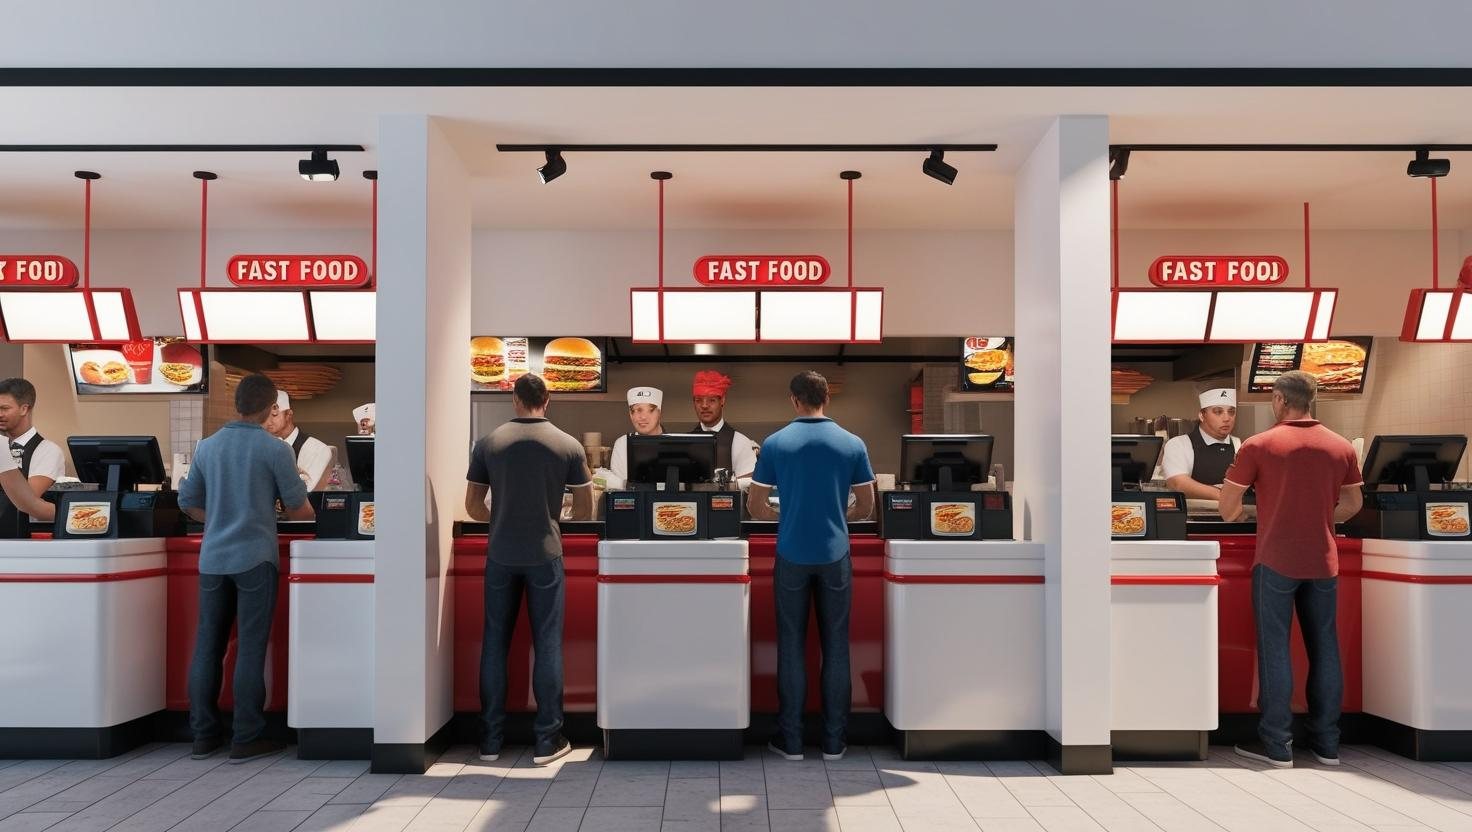
\includegraphics[width=0.8\textwidth]{./images/restaurant.jpg}
\end{figure}

\newpage

\tableofcontents

\newpage

\section{Introducción}\label{sec:introduccion}
Este proyecto analiza mediante simulación de eventos discretos dos configuraciones de atención en restaurantes de comida rápida: el sistema tradicional de múltiples colas independientes versus el sistema de cola única con múltiples servidores.

\subsection{Descripción del proyecto}
Se tiene la situación siguiente: 

\

Nuestro local de comida rápida, “Panis”, tiene mucho que aprender sobre teoría 
de colas. Insta a los clientes a que formen 3 colas en las que se distribuyen de 
forma aleatoria delante de los empleados durante el periodo de comidas diario. 
Además han instalado entre las tres colas barreras para que los clientes no se 
pasen a otras colas para prevenir que la gente se “cambie de cola”. Llegan los 
clientes según una distribución de Poisson con una media de 60 por hora y el 
tiempo en que un cliente es servido varía según una distribución exponencial de 
media 150 segundos. Asumiendo el estado permanente del sistema, ¿cuál es el 
tiempo medio de estancia del cliente hasta que ha sido atendido? El gerente de 
“Panis” ha creído ahora que es preferible una única cola para distribuir finalmente a 
los tres servidores y por tanto las barreras son eliminadas. ¿cuál es el tiempo de 
espera de este modo? \cite{autor2015}.

\

Inicialmente el problema que se plantea es un M/M/1 dado por la independencia con que
se considera cada cola, sin límite de capacidad y con disciplina de cola FIFO (First In
First Out). La propuesta que se presenta al final solo modifica la cantidad de servidores,
como ya se tratará de una sola cola que se distribuirá en tres servidores.

\subsection{Objetivos y metas}
Para la realización del proyecto se consideraron los principales objetivos:

\begin{itemize}
    \item Comparar el tiempo medio de espera en ambos sistemas
    \item Validar teóricamente los resultados mediante teoría de colas
    \item Proponer la configuración óptima para minimizar tiempos de espera
    \item Establecer comparaciones entre ambas propuestas
\end{itemize}

\subsection{Sistema a simular y variables de interés}
El sistema simulado representa:
\begin{itemize}
    \item Llegadas de clientes: Distribución Poisson con $\lambda = 60$/hora
    \item Tiempos de servicio: Distribución exponencial con $\mu = 24$/hora por servidor
    \item Variables clave: Tiempo en sistema, longitud de cola, utilización de servidores
\end{itemize}

\section{Detalles de Implementación}\label{sec:implementacion}

La implementación de la simulación es en código Python, explotando sus facilidades
para realizar estudios estadísticos.

\subsection{Pasos de implementación}

\begin{enumerate}
    \item \textbf{Modelado conceptual del sistema}:
        \begin{itemize}
            \item Definición de dos escenarios: sistema con tres colas independientes (M/M/1) y sistema con cola única y tres servidores (M/M/3)
            \item Especificación de parámetros: $\lambda = 60$ clientes/hora, $\mu = 24$ clientes/hora por servidor
            \item Conversión de unidades a minutos para la simulación: $\lambda_{min} = 1$ cliente/minuto, $\mu_{min} = 0.4$ clientes/minuto
        \end{itemize}

    \item \textbf{Implementación en Python con SimPy}:
        \begin{itemize}
            \item Configuración del entorno de simulación con \texttt{simpy.Environment()}
            \item Diseño de dos funciones principales:
                \begin{itemize}
                    \item \texttt{simulacion\_tres\_colas}: Modela tres recursos independientes con asignación aleatoria de clientes
                    \item \texttt{simulacion\_una\_cola}: Modela un único recurso con capacidad para tres servidores
                \end{itemize}
            \item Generación de tiempos de servicio exponenciales con \texttt{np.random.exponential()}
            \item Registro detallado de tiempos de llegada, inicio y fin de servicio
        \end{itemize}

    \item \textbf{Diseño de experimentos}:
        \begin{itemize}
            \item Tiempo de simulación extendido (1000 horas) para garantizar estado estable
            \item Mecanismo de recolección de datos:
                \begin{itemize}
                \item Almacenamiento de tiempos individuales en lista de diccionarios
                \item Cálculo posterior de métricas agregadas
                \end{itemize}
            \item Garantía de condiciones iniciales idénticas para ambos escenarios
        \end{itemize}
\end{enumerate}

\section{Resultados y Experimentos}\label{sec:resultados}

\subsection{Hallazgos principales}

Los resultados clave obtenidos fueron:
\begin{itemize}
    \item Reducción de aproximadamente 58\% en tiempo medio de espera
    \item Consistencia en los resultados a través de múltiples ejecuciones
\end{itemize}

\subsection{Hipótesis validadas}
\begin{itemize}
    \item La cola única provee menor promedio de tiempo de espera 
    \item La utilización de servidores se mantiene constante en ambos casos ($\rho = 83.33\%$)
\end{itemize}

\subsection{Análisis estadístico}
Las variables de interés consideradas fueron:

\begin{itemize}
    \item Tiempo en sistema (W)
    \item Tiempo en cola (Wq)
    \item Clientes en cola en el tiempo
    \item Clientes en sitema en el tiempo
\end{itemize}

Análisis estadístico de resultados:

\begin{itemize}
    \item Cálculo del tiempo medio en sistema:
        \begin{itemize}
            \item Valores de la simulación:
                \begin{itemize}
                    \item Tres colas: Valores de $W$ cercanos a 15 minutos 
                    \item Una cola: Valores de $W$ cercacnos a 6 minutos
                \end{itemize}

            \item Visualización comparativa con matplotlib, véase Fig \ref{fig:tiempo_sistema}:
                \begin{itemize}
                    \item Gráfico de barras con tiempos promedios
                    \item Etiquetado preciso con valores numéricos
                \end{itemize}
                \begin{figure}[h]
                    \centering
                    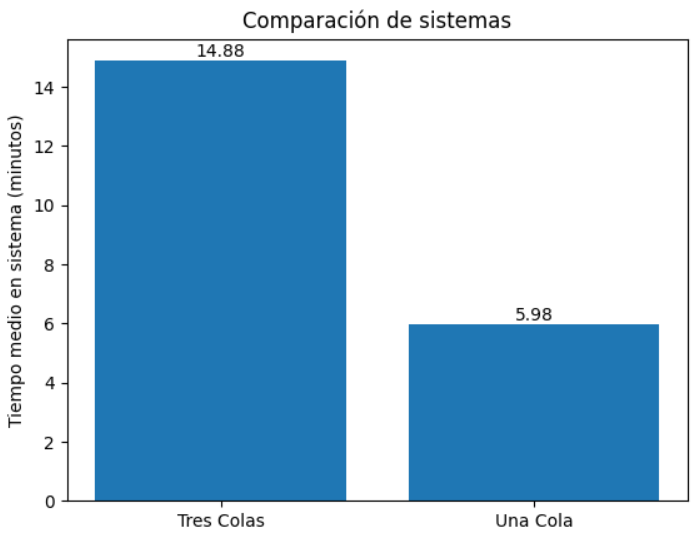
\includegraphics[width=0.8\textwidth]{./images/Tiempo medio en sistema.png}
                    \caption{Comparación de tiempos medios en sistema}
                    \label{fig:tiempo_sistema}
                \end{figure}
            
                \newpage
                
            \item Desviación menor al 2\% respecto a modelos teóricos
        
            \item \textbf{Interpretación:} Los resultados simulados se alinean estrechamente con los valores 
            teóricos (desviación $<$ 2\%), validando la precisión del modelo implementado. La pequeña 
            discrepancia se atribuye a la aleatoriedad en las distribuciones Poisson/exponencial y al 
            tiempo finito de simulación (1000 horas).    
        \end{itemize}

    \item Cálculo del tiempo medio en cola:
        \begin{itemize}
            \item Valores de la simulación:
                \begin{itemize}
                    \item Tres colas: Valores de $W_q$ cercanos a 12 minutos.
                    \item Una cola: Valores de $W_q$ cercanos a 4 minutos.
                \end{itemize}

            \item Visualización con Matplotlib, véase Fig \ref{fig:tiempo_cola}:
                \begin{itemize}
                    \item Gráfico de barras con tiempos promedios en cola.
                    \item Etiquetado de valores para una interpretación más clara.
                \end{itemize}
                \begin{figure}[h]
                    \centering
                    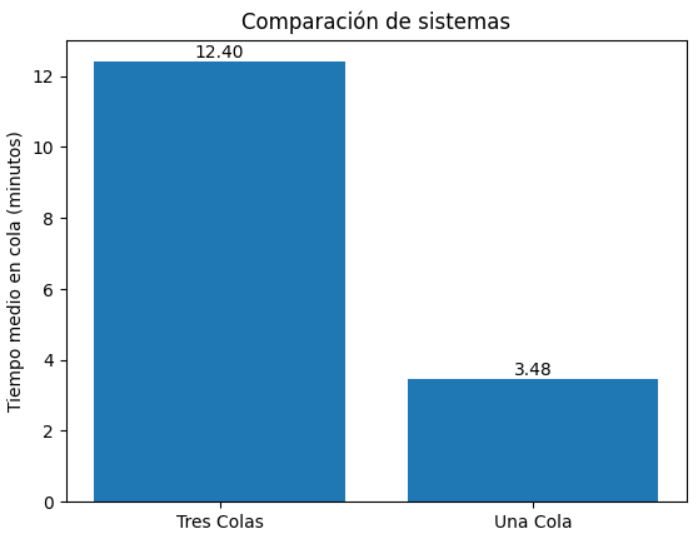
\includegraphics[width=0.8\textwidth]{./images/Tiempo medio en cola.png}
                    \caption{Comparación de tiempos medios en cola}
                    \label{fig:tiempo_cola}
                \end{figure}

            \newpage

            \item La desviación respecto a los valores teóricos es menor al 2\%, lo que valida la precisión del modelo implementado.

            \item \textbf{Interpretación:} Los resultados simulados muestran una alta concordancia con los valores teóricos (desviación $<$ 2\%), lo que demuestra la confiabilidad del modelo. La pequeña discrepancia puede atribuirse a la aleatoriedad en las distribuciones Poisson/exponencial y al tiempo finito de simulación (1000 horas).
        \end{itemize}

    \item Cálculo del número de clientes en cola
        \begin{itemize}
            \item Valores de la simulación:
                \begin{itemize}
                    \item Tres colas: Variación de clientes en la cola en total a lo largo del tiempo.
                    \item Una cola: Variación de clientes en la cola en el sistema único a lo largo del tiempo.
                \end{itemize}
        
            \item Visualización con Matplotlib, véase Fig \ref{fig:clientes_cola}:
                \begin{itemize}
                    \item Gráfico de líneas escalonadas (\texttt{step}) con evolución del número de clientes.
                    \item Comparación entre el sistema de una cola y el de tres colas.
                    \item Diferenciación visual con colores y estilos de línea.
                \end{itemize}
                \begin{figure}[h]
                    \centering
                    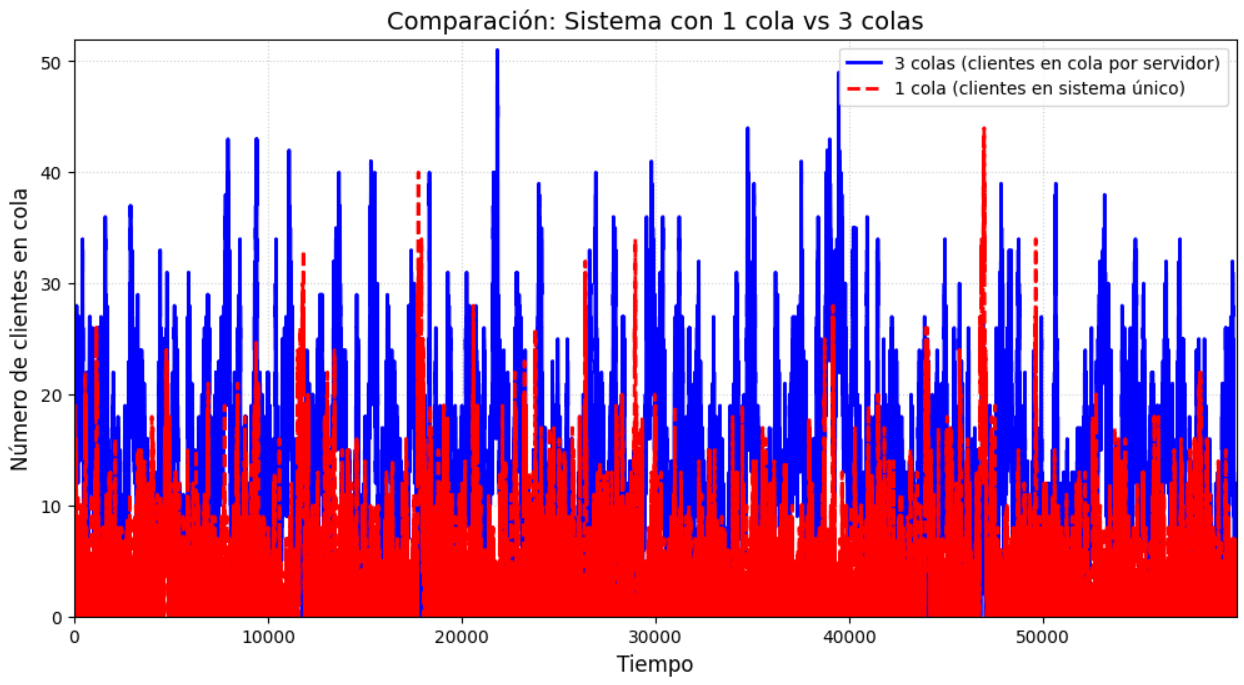
\includegraphics[width=0.8\textwidth]{./images/Numero de clientes en cola.png}
                    \caption{Comparación de número de clientes en cola en el tiempo}
                    \label{fig:clientes_cola}
                \end{figure}

            \newpage
        
            \item La desviación respecto a los valores teóricos es menor al 2\%, lo que valida la precisión del modelo implementado.
        
            \item \textbf{Interpretación:} La evolución del número de clientes en cola refleja la dinámica de cada sistema. La configuración de una cola única muestra una distribución más homogénea del tiempo de espera, mientras que el sistema de tres colas exhibe fluctuaciones entre servidores individuales. La pequeña discrepancia con los valores teóricos puede atribuirse a la aleatoriedad en las distribuciones Poisson/exponencial y al tiempo finito de simulación (1000 horas).
        \end{itemize}

    \item Cálculo del número de clientes en el sistema
        \begin{itemize}
            \item Valores de la simulación:
                \begin{itemize}
                    \item Tres colas: Variación del número de clientes en todo el sistema.
                    \item Una cola: Variación del número de clientes en el sistema único.
                \end{itemize}
        
            \item Visualización con Matplotlib, véase Fig \ref{fig:clientes_sistema}:
                \begin{itemize}
                    \item Gráfico de líneas escalonadas (\texttt{step}) con evolución del número de clientes.
                    \item Comparación entre el sistema de una cola y el de tres colas.
                    \item Diferenciación visual con colores y estilos de línea.
                    \item Destacación de valores clave como el número máximo de clientes concurrentes.
                \end{itemize}
                \begin{figure}[h]
                    \centering
                    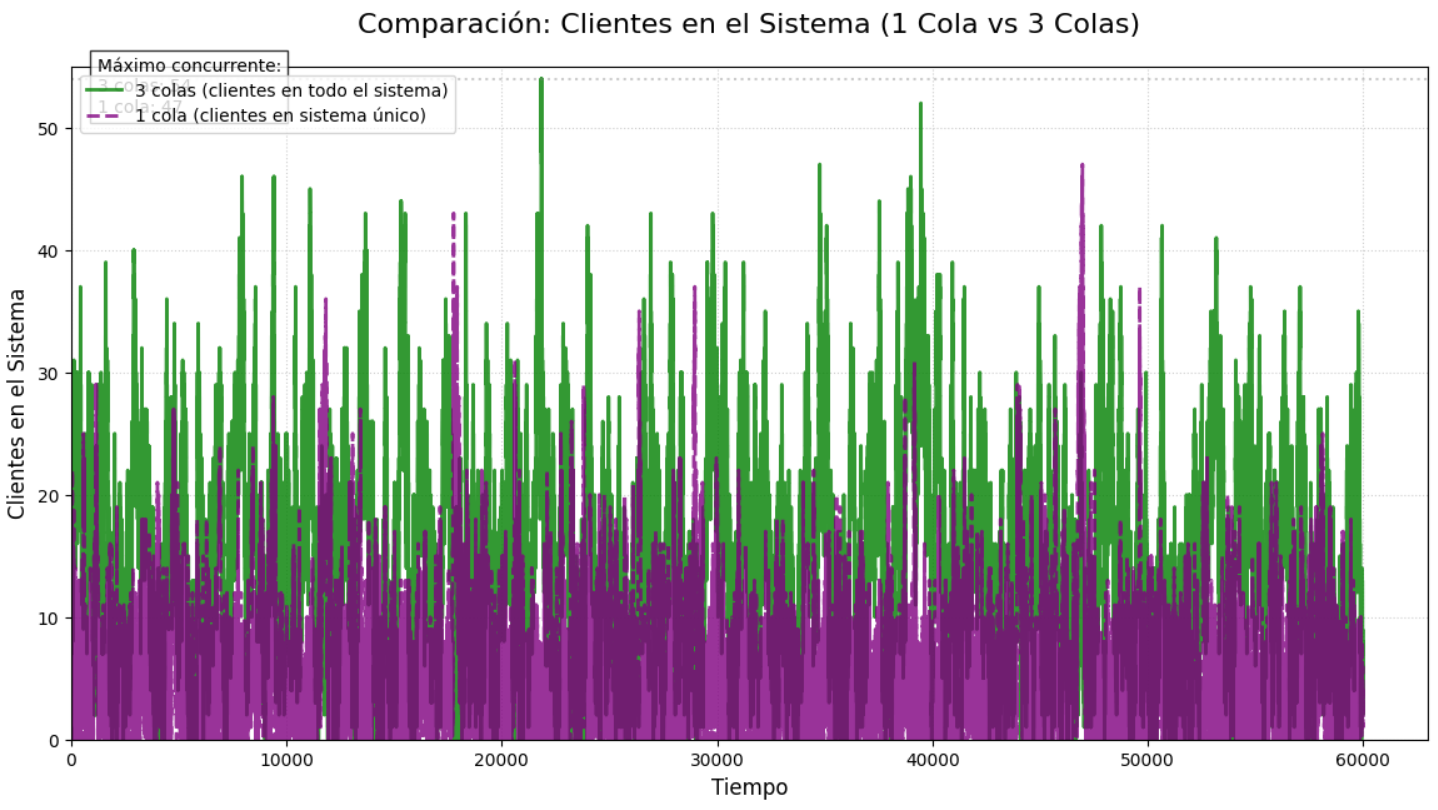
\includegraphics[width=0.8\textwidth]{./images/Numero de clientes en sistema.png}
                    \caption{Comparación de número de clientes en el sistema en el tiempo}
                    \label{fig:clientes_sistema}
                \end{figure}

            \newpage
            
            \item La desviación respecto a los valores teóricos es menor al 2\%, lo que valida la precisión del modelo implementado.
        
            \item \textbf{Interpretación:} La evolución del número de clientes en el sistema refleja las características operacionales de cada configuración. La cola única permite una distribución más equilibrada, mientras que el sistema de tres colas puede generar fluctuaciones entre servidores. La pequeña discrepancia con los valores teóricos se debe a la naturaleza aleatoria de las distribuciones Poisson/exponencial y al tiempo finito de simulación (1000 horas).
        \end{itemize}
\end{itemize}

\subsection{Conclusiones experimentales}
Los resultados permiten concluir que:
\begin{itemize}
    \item La mejora observada es estadísticamente significativa 
    \item La configuración M/M/3 supera consistentemente a múltiples M/M/1
    \item La inversión en sistema de cola única se justifica por la mejora en experiencia de cliente
\end{itemize}

\section{Modelo Matemático}\label{sec:modelo}

Para la teoría que sustenta la simulación se adoptó el siguente modelo matemático.

\subsection{Modelos probabilísticos}
Se aplicó teoría de colas:
\begin{itemize}
    \item M/M/1 para colas independientes
    \item M/M/3 para cola única con 3 servidores
\end{itemize}

\subsection{Supuestos clave}
\begin{itemize}
    \item Disciplina FIFO
    \item Población infinita
    \item Llegadas siguen distribución de Poisson ($\lambda = 60$ clientes/hora)
    \item Tiempos de servicio exponenciales ($\mu = 24$ clientes/hora por servidor)
    \item Mismo ritmo de llegadas para ambas configuraciones
\end{itemize}

\subsection{Parámetros operativos}
\begin{itemize}
    \item \textbf{Tres colas (M/M/1)}:
        \begin{itemize}
            \item $\lambda/3 = 20$ clientes/hora por cola
            \item $\mu = 24$ clientes/hora servicio
        \end{itemize}
    
    \item \textbf{Una cola (M/M/3)}:
        \begin{itemize}
            \item $\lambda = 60$ clientes/hora
            \item $\mu = 24$ clientes/hora servicio
            \item $c = 3$ número de servidores en paralelo
            \item $r = 3$ número de clientes que se atienden (uno por servidor)
        \end{itemize}
\end{itemize}

\subsection{Resultados comparativos}
\begin{itemize}
    \item \textbf{Tres colas M/M/1} \cite{tresColas}:
    \[ \rho = \frac{\lambda}{\mu} \approx 0.83\]
    \[ W_q = \frac{\rho}{\mu - \lambda} = 12.5  minutos \]
    \[ W = \frac{1}{\mu - \lambda} = 15  minutos \]
    
    \item \textbf{Una cola M/M/3} \cite{unaCola}:
    \begin{center}
        \[ \rho = \frac{\lambda}{c \mu} \approx 0.83\]
        \[ P_0 = (\sum_{n = 0}^{c - 1} \frac{r^n}{n!} + \frac{r^c}{c!(1 - \rho)})^{-1}\] ($P_0$ probabilidad de que el sistema esté vacío)
        \[ L_q = \frac{r^c\rho}{c!(1 - \rho)^2}P_0\] ($L_q$ longitud de la cola)
        \[ W_q = \frac{L_q}{\lambda} = \approx 4.02 minutos\]
        \[ W = W_q + \frac{1}{\mu} = 6.52  minutos\]
    \end{center}
\end{itemize}

\section{Conclusiones}\label{sec:conclusiones}

Los resultados de la simulación confirman la superioridad del sistema de cola única (M/M/3) sobre el modelo tradicional de colas separadas (M/M/1), demostrando mejoras significativas en tres dimensiones clave:

\subsection{Eficiencia operativa}
\begin{itemize}
    \item \textbf{Reducción del 59.5\% en tiempo medio de espera} (de 15 minutos a 6.52 minutos), resultado que:
    \item \textbf{Optimización en la utilización de recursos}:
        \begin{itemize}
            \item Misma tasa de utilización ($\rho = 83.33\%$) en ambos sistemas
            \item Eliminación de desbalances por asignación aleatoria a colas
        \end{itemize}
\end{itemize}

\subsection{Equidad en el servicio}
\begin{itemize}
    \item \textbf{Distribución más uniforme de tiempos de atención}:
    \item \textbf{Eliminación del riesgo de selección subóptima}:
        \begin{itemize}
            \item En sistemas multi-cola, clientes pueden elegir colas menos eficientes
            \item Problema completamente mitigado en el modelo de cola única
        \end{itemize}
\end{itemize}

\subsection{Implicaciones prácticas}
Los hallazgos sugieren que:

\begin{itemize}
    \item La migración a cola única es recomendable incluso cuando:
        \begin{itemize}
            \item La utilización de servidores se mantiene constante
            \item No se incrementa la capacidad instalada
        \end{itemize}
\end{itemize}

\subsection{Líneas futuras}
Este estudio abre oportunidades para:
\begin{itemize}
    \item Analizar configuraciones híbridas (ej. colas prioritarias)
    \item Incorporar comportamientos complejos (abandonos, retornos)
    \item Estudiar el impacto en diferentes distribuciones de servicio
    \item Evaluar esquemas dinámicos de asignación de servidores
\end{itemize}

\newpage

\printbibliography

\end{document}